% %%novalidate

\usepackage{tikz}
\usepackage{calc}
\usepackage{booktabs}
\usepackage[hidelinks]{hyperref}

% colors
\definecolor{color1}{HTML}{000060}
%\definecolor{color1}{HTML}{8C260F}
\definecolor{color2}{HTML}{333333}


% fonts
\usepackage{fontspec}
\defaultfontfeatures{Mapping=tex-text}
\setmainfont
[BoldFont=Lato-Bold.ttf,
ItalicFont=Lato-Italic.ttf,
BoldItalicFont=Lato-BoldItalic.ttf]
{Lato-Regular.ttf}
\newfontfamily\headingfont[ItalicFont=Lato-BlackItalic.ttf]{Lato-Black.ttf}
%%%

\usepackage{geometry}
\geometry{a4paper,
hmargin=15mm,vmargin=20mm,
head=0ex,foot=3ex}

\linespread{1.3}

\usepackage[hang]{caption}
\DeclareCaptionFormat{upper}{#1#2\uppercase{#3}\par}
\captionsetup{labelfont={bf,color=color2},textfont={normalsize,color=color2},format = upper,figurename=FIGURE,tablename=TABLE}

%%% fancy sections
\usepackage{titlesec}
% \titleformat{\chapter}{\headingfont\LARGE\bfseries\scshape\color{color1}}{\thechapter}{1em}{}[\titlerule]
\titleformat{\section}{\color{color1}\headingfont\Large\bfseries\uppercase}{\thesection}{1em}{}[\titlerule]
\titleformat{\subsection}{\color{color1}\headingfont\large\bfseries\uppercase}{\thesubsection}{1em}{}
\titleformat{\subsubsection}{\color{color1}\headingfont\bfseries\uppercase}{\thesubsubsection}{1em}{}
%%%

% head and foot
\usepackage{fancyhdr}
\pagestyle{fancy}
\lhead{}
\chead{}
\makeatletter
% \rhead{\color{color2}\@date}
\rhead{}
\makeatother
\newlength{\myheight}
\lfoot{
\settoheight{\myheight}{\thepage}
\raisebox{-2ex-1.5\myheight}{
\includegraphics[height=5ex]{logo}}
}
% \cfoot{\color{color2}\LaTeX\ template for business reports}
\cfoot{}
\rfoot{\color{color2}\thepage}
\renewcommand\headrulewidth{0pt}
\renewcommand\footrulewidth{0pt}

%%% picture on cover page
\usepackage{eso-pic}
\newcommand\BackgroundPic{%
\put(0,0){%
\parbox[b][\paperheight]{\paperwidth}{%
\vfill
\centering
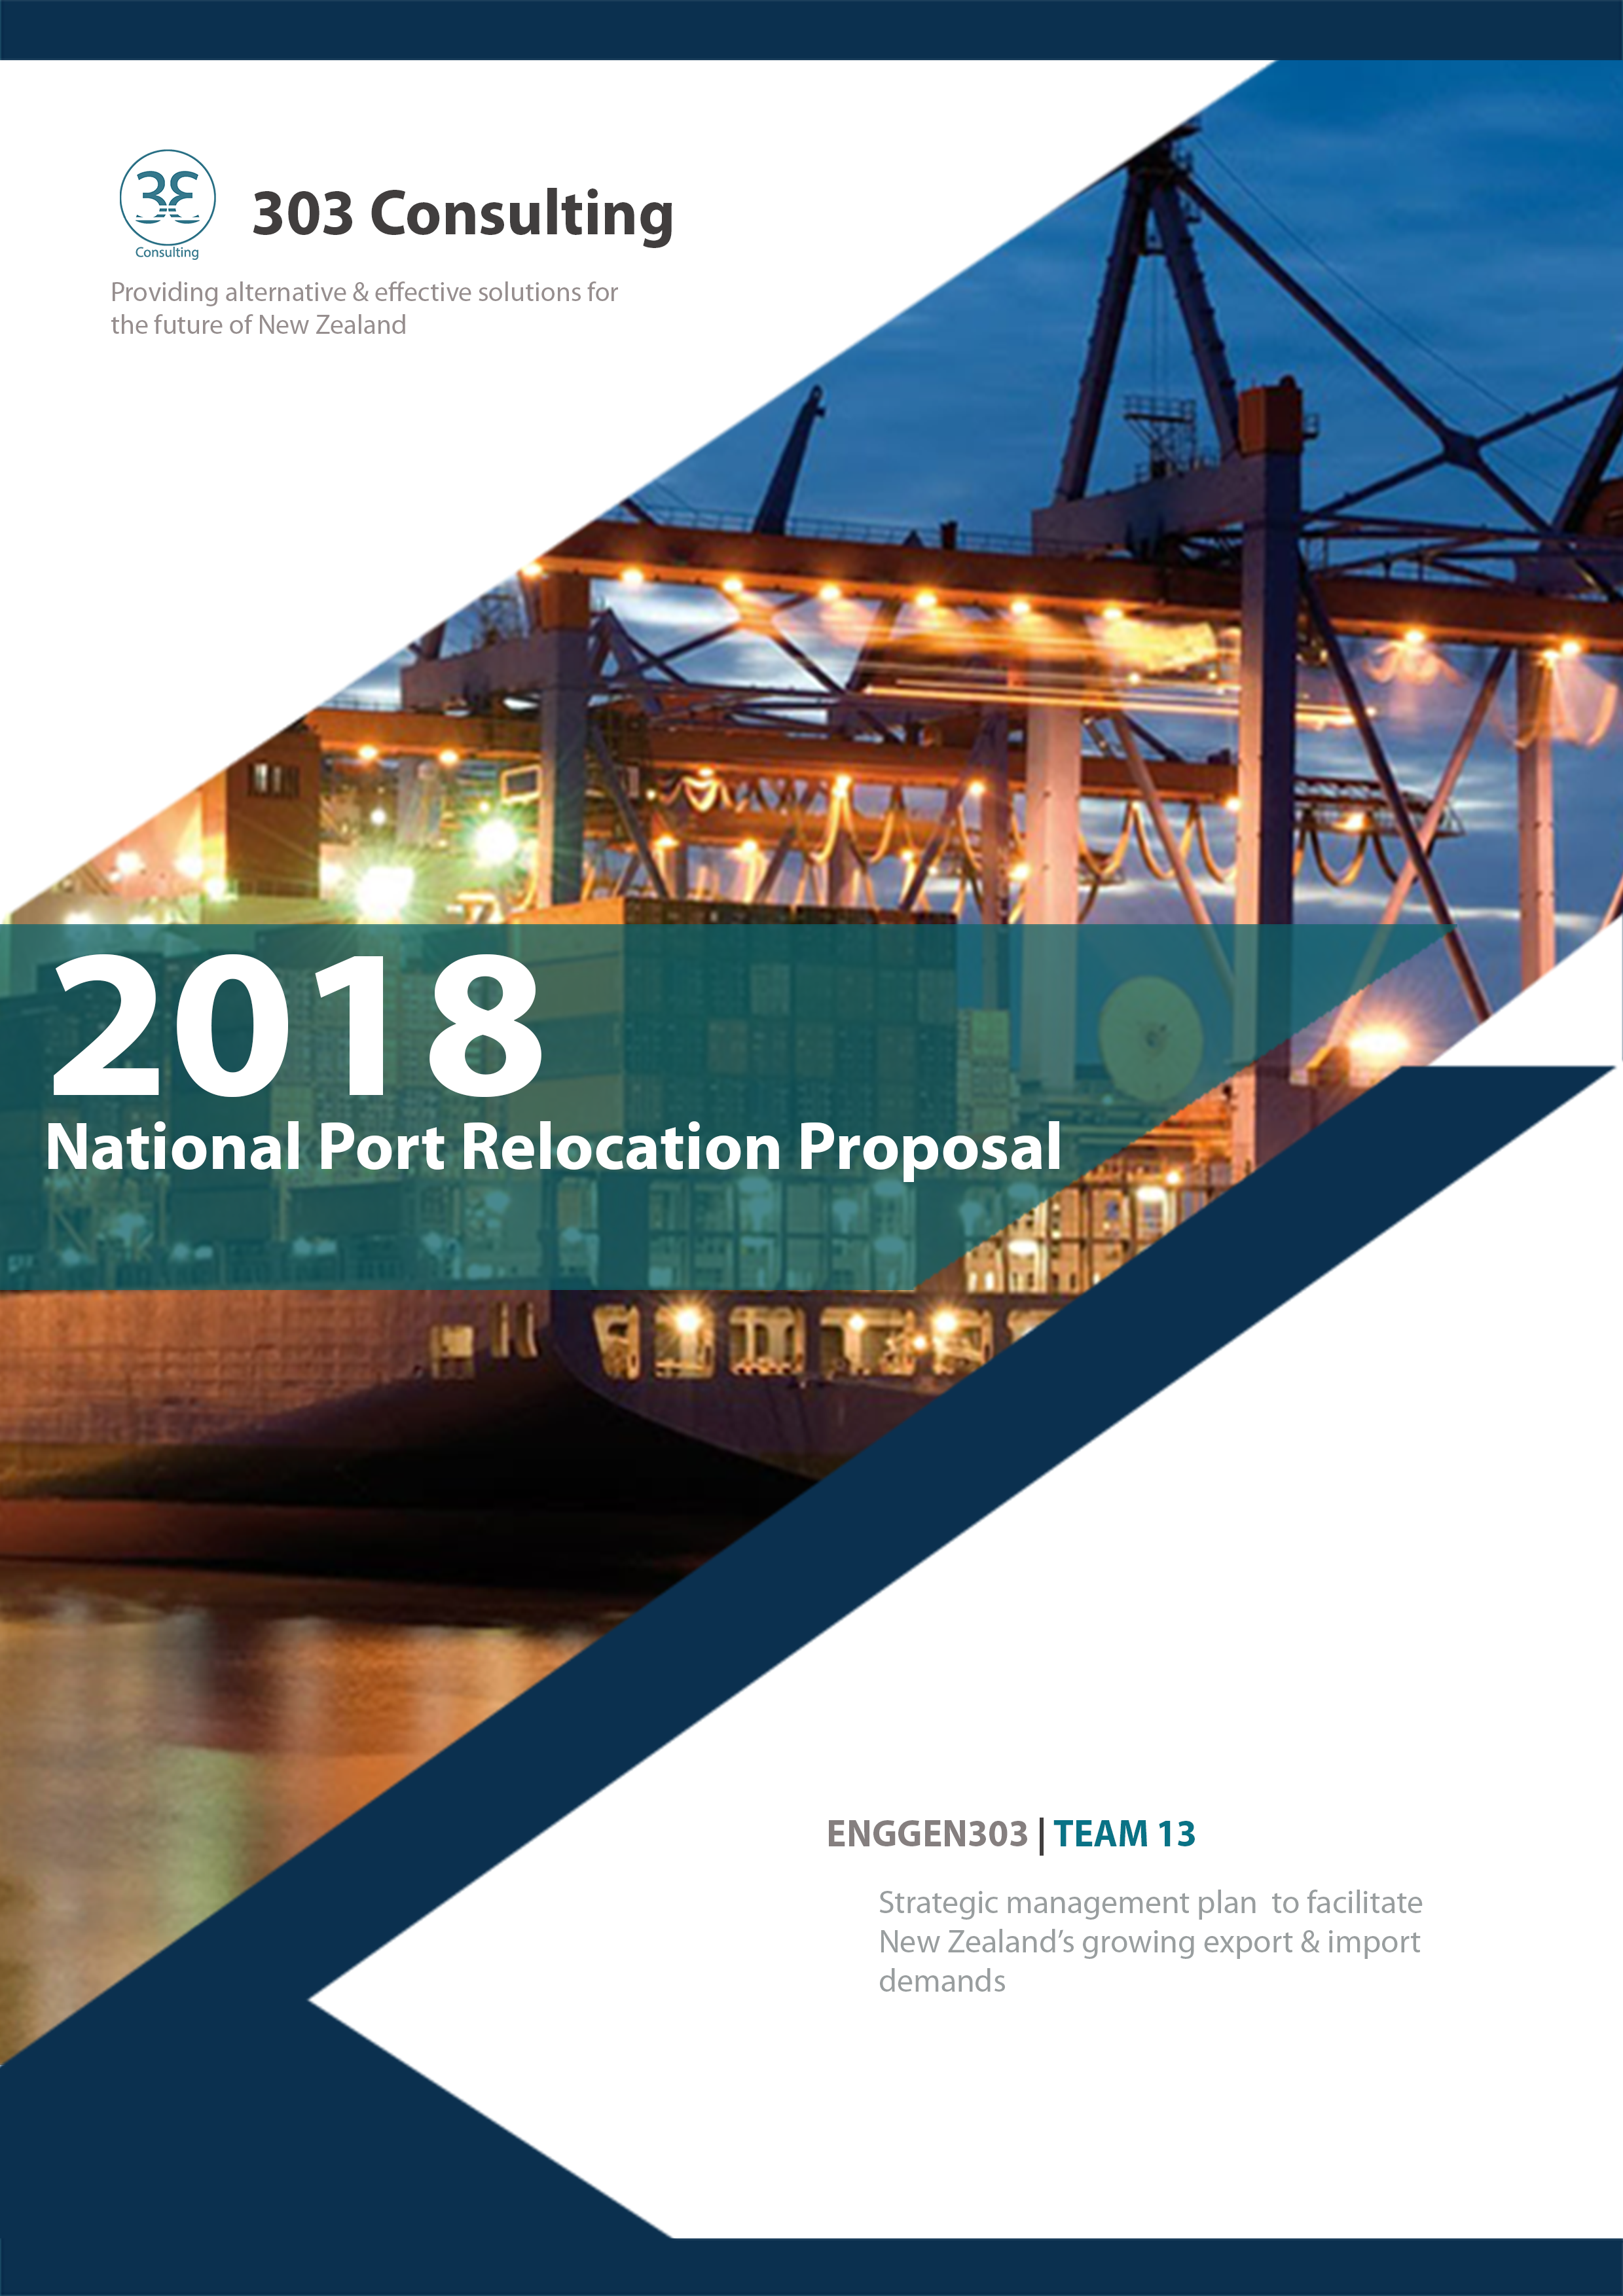
\includegraphics[width=\paperwidth,height=\paperheight,%
keepaspectratio]{cover}%
\vfill
}}}
%%%
% custom titlepage
\makeatletter
\renewcommand{\maketitle}{
\thispagestyle{empty}
\AddToShipoutPicture*{\BackgroundPic}
\ClearShipoutPicture
%
\phantom{a}
\vfill
% \phantom{a}\hfill
\begin{tabular}[c]{@{}p{\textwidth}@{}}
    %   \color{white}\headingfont\LARGE\@title\\[1em]
    %   \color{white}\headingfont\Large\@author\\[3em]
\end{tabular}
%
\clearpage
}
\makeatother
%%%


%%% fancy boxes
\usepackage{tcolorbox}
\usepackage{wrapfig}
\def\fullboxbegin{
\bigskip
\begin{tcolorbox}[colback=color1,colframe=color1,coltext=white,arc=0mm,boxrule=0pt]
}
\def\fullboxend{\end{tcolorbox}\medskip}
%
\def\leftboxbegin{
\begin{wrapfigure}{l}{0.5\textwidth}
\begin{tcolorbox}[colback=color1,colframe=color1,coltext=white,arc=0mm,boxrule=0pt]
}
\def\leftboxend{
\end{tcolorbox}
\end{wrapfigure}
}
%
\def\rightboxbegin{
\begin{wrapfigure}{r}{0.5\textwidth}
\begin{tcolorbox}[colback=color1,colframe=color1,coltext=white,arc=0mm,boxrule=0pt]
}
\def\rightboxend{
\end{tcolorbox}
\end{wrapfigure}
}
%
\newcounter{frames}
\def\frameboxbegin#1{
\bigskip
\refstepcounter{frames}
\begin{tcolorbox}[colback=white,colframe=color1,arc=0mm,title={\MakeUppercase{\textbf{Frame \arabic{frames}}: #1}}]
}
\def\frameboxend{
\end{tcolorbox}
}
%%%

\newcommand{\imgsection}[2]{
%   \refstepcounter{section}
  \newgeometry{top=0cm}
%   \addcontentsline{toc}{section}{\protect\numberline{\thesection}#1}
%   \sectionmark{#1}
  \begin{center}
  \makebox[\textwidth]{\includegraphics[width=\paperwidth]{#2}}
  \end{center}
%   {\normalfont\huge\bfseries
%   \thesection:  #1}
  \restoregeometry
}

\newpage
\refstepcounter{section}
%Add Image
\vspace*{-40mm} %Make image have no top margin
\begin{tikzpicture}
\node[inner sep=0pt] (x) at (0,0)
    {\hspace{-87mm}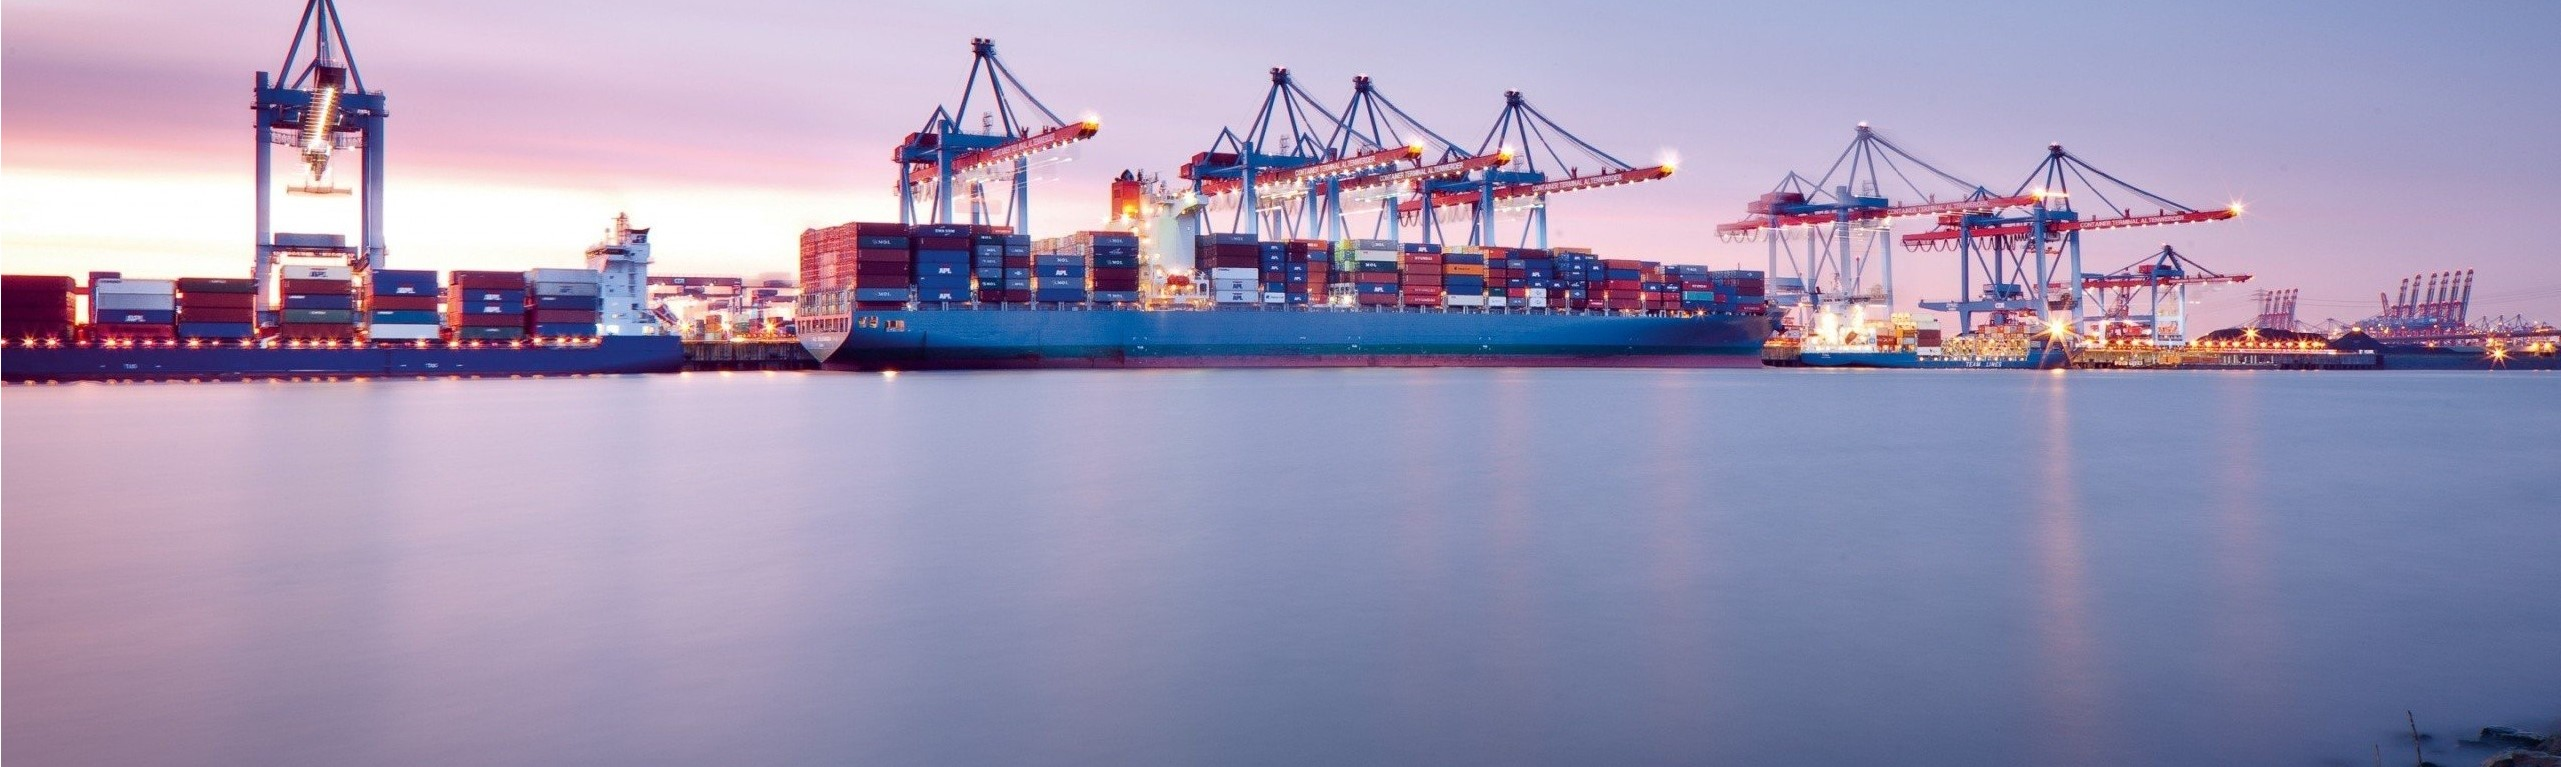
\includegraphics[width=\paperwidth]{sectionimage3.jpg}};
\node[text width=10in] (Z) at (0,-1) {\color{white}\headingfont\Large\bfseries\uppercase{\hspace{-0.7cm}\thesection\hspace{0.5cm}Introduction}};
\end{tikzpicture}
%Modify TOC
\addcontentsline{toc}{section}{\protect\numberline{\thesection}Introduction}
  \sectionmark{Introduction}
\vspace{-2mm}

%Content
\subsection*{Background}
Auckland, known as the City of Sails, has one of the most illustrious views overlooking the Hauraki Gulf from downtown. From daily ferry services to luxury cruise ships, PoA has seen it all. As ships become larger, there is a concern regarding the infrastructure of the PoA is able to handle large volumes of goods imported and exported in the foreseeable future.
\\ Deputy Prime Minister of New Zealand, Hon Winston Peters, suggested during the election campaign that the PoA should be relocated to Whangarei which was agreed upon by the coalition government with Labour. As the demand for freight continues to grow, ports are required to develop their current facilities to cope with change. The PoA is soon to reach maximum operating capacity and will not be able to meet demand of freight. It currently occupies a lot of land which may provide alternative economic growth for Auckland. In addition, reducing container trucks near PoA will ease congestion of downtown traffic. 

\subsection*{Scope}
The scope for this project is to devise a plan for any long term potential relocation of the PoA. It is important to address any stakeholder conflicts the project may incur when in development. The overall cost of the project must be maintained within budget, whilst meeting health and safety, and environmental regulations. The relocation of the port is expected to occur over a 25-year period with at least 20\% still operating at PoA.

\subsection*{Goals}
This project is to determine whether a relocation of the POA is able to be implemented while meeting necessary stakeholder requirements and follow an economically feasible budget. To be successful the project must result in a more efficient and capable freight processing and distribution system which is able to handle the increase in freight quantity in the future.

\clearpage